\chapter{Introduction}

\section{What is Synthetic Biology?}

% life and parts description

Synthetic biology is the design and study of artificial living
organisms, re-engineered organisms, and engineered parts for existing
organisms. The idea is to bring engineering tools and methodologies to
the subject of biology, much as electrical engineering brings these
tools to physics, with the goal of designing novel and useful
biological systems. These novel systems, new life forms really, may
someday afford humanity a new level control over the processes in our
bodies, in our crops, in landfills, compost heaps, and the ocean
waters: Instead of controlling the living world with machines and
harsh chemicals, synthetic biology promises control at the level of
individual molecules using engineered living cells as tiny chemical
processing plants.

Of course, biology is more than just chemical processing. It is
information processing. The instructions for how to grow and regulate
a human being are encoded by the DNA inside each of the cells in your
body. Growth and development follows precise, distributed, robust
algorithms. The immune system can adapt itself to pathogens it has
never seen. A predator can track its prey and outsmart it. Our brains
can do research and write books. Life {\em is} computation. The
molecules and structures inside cells are the tools that nature uses
to implement life's computations, just as the silicon and wires inside
your computer implement computations. Thus, to some
extent, biology (synthetic or otherwise) ought to be seen more
abstractly than our high-school biology books would have us see
it. Our job as living system engineers is to define the abstractions,
the composable modules, the signal carriers, the simplifications, the
programming languages, and the debugging tools for living systems.

We are far from being able to engineer entirely new life forms,
although remarkable advances are being made every day. Many of these
advances are technological, such as rebooting cells so that they
become stem cells \cite{reprogramming}, putting the genome of one cell
into another \cite{cloning}, synthesizing large pieces of DNA
\cite{m-genetalium}, and improved methods for tracking molecules
inside cells \cite{fret-in-cells}. Other advances are more conceptual,
such as new understandings of stochastic chemical kinetics
\cite{khammash-fsp,el-samad-stochastic}, system identification feedback
control inside cells \cite{avano-osmotic}, directed evolution
\cite{alon}, and so on. Perhaps most telling, some advances look like
hacking: artificial oscillators inside cells
\cite{elowitz-repressilator}, engineered cell-cell communication
\cite{weiss-communicate}, digital logic inside cells
\cite{weiss-logic}. The fact that researchers in well-equipped labs
and others in their garages \cite{diy} can now make their own widgets
for living systems suggests that the technologies for and the
conceptual understandings of living systems are now sufficiently rich
to allow engineers to to tinker. And tinkering leads to engineering
research, which leads to engineering practice.

% practical description: sensing, control, actuation, information, evolution
It is fun to argue about what life {\em is} or what it would mean to
actually have built a living organism or enough of one to call it a
truely new species. However, in this book we will take a more
pragmatic approach and look, instead, at what living systems seem to
know how to do well: sense, actuate, control, process information, and
evolve. These five capabilities -- present in all the living systems
we can think of -- are probably necessary for all life forms, and in
this book we focus mainly on them as goals for what to
build. Furthermore, these capabilities, except for the last one, are
usually thought of by engineers as the important aspects of embedded
control systems (such as automobiles or cell phones). We hope to use
our experience engineering embedded systems for engineering living
systems, an idea that leads to the question: What do we mean by
sensing, actuation, control, and information processing in the context
of living systems?

%
% Should there be a formal definition of a sensor?
%  
\paragraph{Sensing:} A cell can sense all sorts of quantities, inside
itself and outside. For example, the bacterium {\em E. coli} makes a
protein called {\em LacI} (for {\em lactose inhibitor}) that changes
shape in the presence of the sugar lactose. This has downstream
effects that change the cell's metabolic machinery so that it can
efficiently digest lactose \cite{lac-operon}. Essentially, {\em LacI}
{\em senses} the presence of lactose. In fact, all cells have
molecular mechanisms that can sense the small molecules normally found
in nature, as well they should. Some of these molecules are nutrients,
some are toxins, some represent signals from other cells, and so
on. Any organism that has a good estimate of what is happening in its
environment has an advantage over less ``aware'' organisms. There are
also cells that can sense temperature \cite{heat-shock}, acidity
\cite{ph-sensor}, light \cite{light-sensor}, magnetic fields
\cite{magnetosome}, and on and on. Synthetic biologists use these
capabilities, often by putting the gene for a type of sensor found in
one organism into a genetic regulator circuit being engineered in
another, thereby giving their system new capabilities. For example,
synthetic biologists have put arsenic sensors in {\em E. coli} to make
a device that can warn users of tainted water \cite{arsenic-sensor}.

%
% NOTE: using polaroid distance sensors in robots
%

%
% Should there be a definition of an actuator?
%
\paragraph{Actuation:} A cell can alter its environment, or itself, in
a variety of ways. It can emit a small molecule as a signal to other
cells. Many cells, such as {\em E. coli}, can move by swirling their
flagella while other cells, such as amoebae, move by growing and
digesting their cytoskeletons. Internally, cells can synthesize a wide
variety of molecules that can have huge effects on the cell and its
environment. In fact, {\em making something} is a form of actuation. A
newly synthesized molecule, such as a protein, can effect structure,
metabolism, signaling within and outside of the cell, and so on. Once
again, synthetic biologists borrow the actuators from other organisms
(or make their own) and hook them up to sensors in novel ways to
create new behaviors. For example, a widely used actuator is {\em
  green fluorescent protein} (GFP) \cite{gfp}, which is a molecule
usually found in jellyfish that happens to fluoresce. Synthetic
biologists use GFP like embedded systems engineers use light emitting
diodes, as indicators that something has changed inside the cell. For
example, the arsenic sensor mentioned above is coupled to GFP
production so that cells that detect arsenic glow green under
ultraviolet (dark) light.

\begin{figure}
\centering
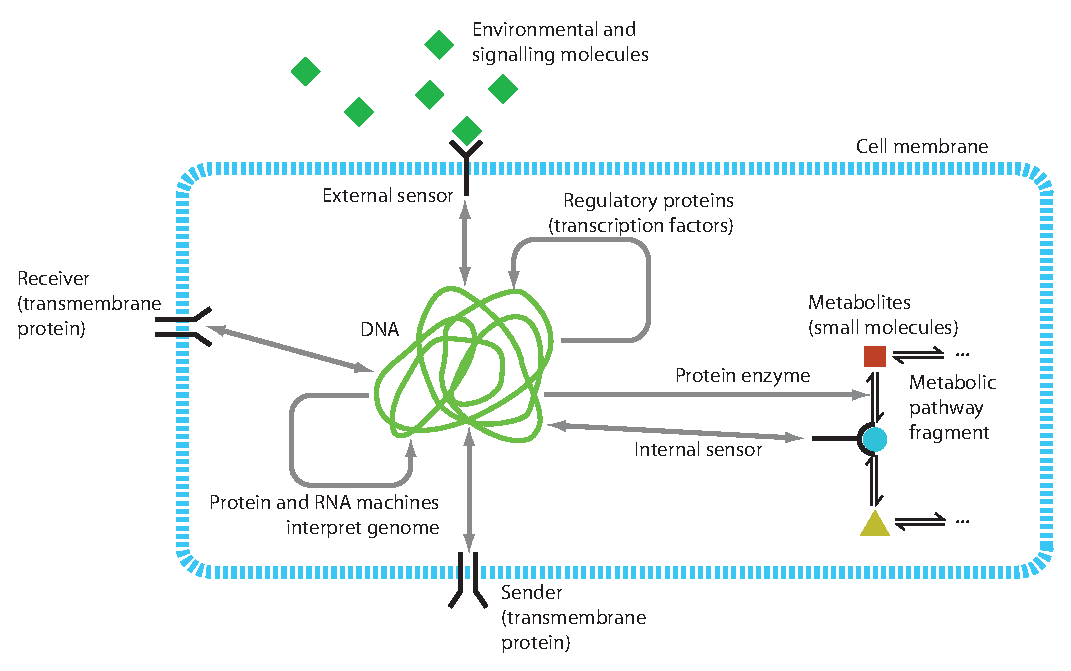
\epsfig{file=figures/cell.eps, scale=0.7}
\caption{\label{fig:thecell} The general structure of a sensing,
  control, actuation and information in the cell. Small molecules can
  be sensed with transmembrane proteins. Internal small molecules can
  be sensed with other sensing proteins. Other controllable
  transmembrane proteins can shuttle molecules in or out of the
  cell. Enzymes control the rates of reactions among metabolites. All
  of this activity is orchestrated by protein and RNA machines that
  interpret the a program stored in the DNA.}
\end{figure}

\paragraph{Control:} Many aspects of a cell's behavior need to be
regulated. Biologists usually call the process by which the
concentrations of various important molecules are regulated {\em
  homeostasis}. Good control requires feedback, which requires sensing
and actuation. For example, yeast cells have control circuits for {\em
  osmotic pressure} \cite{avano-osmotic}, which work by (1) sensing
the osmotic pressure difference across the cell membrane using a very
elegant molecular sensor; and (2) changing the rate at which they pump
glycerol out of the cell, by activating more ``pumping'' proteins. The
system involves many types of molecules interacting in complex ways,
but the net effect is that the osmotic pressure system behaves like a
second order, integral-feedback controller.  Organisms regulate many
other things as well. Your body regulates blood-pressure,
blood-glucose concentration, heart-rate, fat, balance, and many other
important variables. Control of these quantities is important for living
systems primarily because the environment is highly uncertain and,
thus, cannot be relied upon to supply steady levels of any important
variables; cells must regulate these things themselves. Synthetic
biologists need to do essentially the same thing with their engineered
systems -- otherwise their engineered systems will be highly sensitive
to the environment and, more pervasive, to their uncertainty about
exactly how the molecules in the system interact.

It turns out that the main difficulty in engineering control systems
inside cells is in implementing a given mathematical control law using
only the biochemical parts available, which are few and poorly
characterized at best. With electronics, and especially computers,
control engineers have become accustomed to easy implementations of
complex mathematical control algorithms. But with synthetic biology, a
whole new {\em controller synthesis} technology must be developed. This
{\em new synthesis} is a topic of intense research, is by no means
complete, and is the main subject of this book.

\paragraph{Information:} Information is stored and processed on many
levels in a cell. For example, the DNA in a cell stores the
instructions for how to build and regulate all of the systems
comprising the cell. It very carefully maintains this information and
passes it to its offspring. It is a remarkable fact that almost any
cell in your body can, in principle, be used to grow a new you. Also,
at any given time, a cell has a {\em state} (for example, dividing or
not, growing or not, etc.) that is carefully maintained so that all
subsystems ``know'' the state of the cell. For example, your liver
cells are in different cellular states than your brain cells
(hopefully). Furthermore, information is communicated from cell to
cell via signals. Neurons use electrochemical signals and pituitary
gland cells use protein hormones to send powerful signals all over
your body. A most remarkable information processing system is the
immune system (of, for example, humans) which can tell self from
non-self based on, essentially, the information content of the
molecules the immune system cells encounter. It does this both through
innate and learned responses to information.

Management (and mismanagement) of information inside cells is
essential for modern living organisms. Synthetic biologists have yet
to really tap into information processing in synthetic systems. Yet
having recently learned to engineer information systems (for example,
the Internet), we are eager to engineer information processing systems
for cells: almost every disease imaginable is essentially a problem of
information (stored in bits of foreign DNA) getting into the wrong
places and co-opting existing information processing systems.
%
% viruses?
%

\paragraph{Evolution:} Engineers have not had to deal with technologies
that self-replicate. We simply have never built anything so
complicated. However, synthetic biologists are now tweaking existing
organisms by inserting new functionalities, creating essentially new
strains of the organism. These organisms {\em do} self-replicate and,
therefore, populations of them do {\em evolve}. That living systems
are capable of evolution is what makes them so incredibly robust to
changing environments and competition from other organisms. In fact,
the architecture of life seems even to have evolved the ability to
evolve \cite{evolvability}! For example, some genes are copied with
more errors than others during replication and some genes are less
sensitive to mutations than others \cite{gene-amplification}. This
quality directs genetic experimentation to less essential functions,
producing distributions of offspring some of which are possibly more
fit while all are still viable.

Synthetic biologists have to think about evolution for several
reasons. First, it is usually the case that a synthetically introduced
``feature'' in a cell (such as an arsenic detector-indicator circuit)
exerts a huge metabolic load on the host cell. Any cell that happens
to drop the circuit, therefore, has a considerable selective
advantage. How to build circuits that don't simple evolve away in a
few generations is a huge problem
\cite{carlton-endy}. Second,
introducing a new functionality into a cell and putting a population
of said cells into a new environment creates a new ``starting point''
for evolution \cite{fast-cheap}. Due to our limited
understanding of evolutionary dynamics and ecology, we really have no
idea what will happen to subsequent generations of engineered cells
and are therefore subjecting ourselves to unknown risks. Third,
synthetic biologists may be able to {\em use} evolution to tune
engineered systems, if they can tie the performance of the system to
some metabolic benefit. This opens up the possibility of a design
paradigm wherein we build a circuit that behaves in essentially the
right manner, and then tune it into place using evolution.

%Most probably the new population will be
%out-competed by existing organisms -- but the incredible selective
%pressure on the new population may actually increase the rate at which
%the population evolves.

\section{The Applications of Synthetic Biology}

Engineers often reply to claims that we can make linear amplifiers or
Boolean logic circuits out of molecules with: {\em Why would you want
  to do that? We can already make very good amplifiers out of silicon
  and metal.} While that is true, it isn't very easy to integrate
electronics with living systems. Synthetic biology is not about using
engineered cells in situations for which computers, cell phones,
pacemakers, and microchips are ideally suited. Rather, it is about
finding new applications that interface with living systems using the
technology of living systems. 

In fact, we already apply engineered living systems to all sorts of
problems, if you count domesticated animals and bred and hybrid
plants. Furthermore, herbicide-resistant soybeans, tomatoes that don't
rot, rice with extra vitamins \cite{transgenic-crops}, and a host of
other genetically engineered foods can be found in supermarkets
today. Even more, genetic engineers have harnessed the
protein-production capabilities of micro-organisms to make medicines
for diseases from arthritis \cite{arthritis-protein} to malaria
\cite{artemisinin}. For example, insulin is a protein hormone used to
treat diabetes. It signals the body's cells to take up glucose from
the blood. In the past, insulin was laboriously extracted from pig
pancreases. Several decades ago, however, the gene for insulin was
successfully inserted into bacteria or yeast, which can be grown in
fermentors to produce cheap, high-quality insulin
\cite{insulin-bact,insulin-yeast}. Many other molecules can now be
made in bacteria or yeast as well -- from anti-malarial drugs
\cite{keasling-art} to artificial sweeteners \cite{aspartamene}.

Most of these examples are of {\em genetic engineering}, from which
synthetic biologists (attempt to) distinguish themselves: While
genetic engineering concerns swapping genes among organisms, {\em
  synthetic biology is the construction of entirely new
  systems\footnotemark}. To explore the potential applications of
synthetic biology, we need to find situations in which a system
consisting of a molecular sensor, an actuator, and a control mechanism
would be of use. In this sense, genetic engineering might be
considered first-generation synthetic biology -- in that it usually
deals only with actuators, typically molecule production and
secretion. Control engineers call such systems {\em open loop}. If we
start closing the loop, we then ask: what would be possible if we
could put a bit of computation in genetically engineered systems? The
following is a very short discussion of possible applications, many of
which are already under scrutiny by somebody somewhere. We have
attempted to speculate on what might be possible with more control
engineering in these applications. Many, many other applications have
yet to be imagined.

\footnotetext{Genetic engineers and metabolic engineers often take
  umbrage at such distinctions and the very term {\em synthetic
    biology} is oft-criticized as nothing more than a re-branding of
  existing work. In this text, we will try not to make get involved in
  this argument. We could have easily called the book {\em a systems
    approach to genetic engineering}. The emphasis is on systems
  engineering and engineering living systems. Call it what you like.}

% applications ideas: gene-therapy, biofuel production, carbon
% sequestration, DNA vaccines, materials (e.g. plastic), cheap,
% nutritious food, sensor-detectors, photosynthetic stuff, tools for
% systems bio, bio-remediation (e.g. plastic eaters)

\paragraph{Gene Therapy:} Pharmaceuticals are typically substances
that diffuse throughout the body, hopefully interacting with desired
target cells, but also interacting with everything else. For example,
the drug AZT is intended to interfere with a certain step in the
replication of the HIV virus \cite{azt}. Unfortunately, it also
interferes with a number of other natural processes in the body, and
therefore causes all sorts of side effects. The idea of gene therapy,
in contrast, is to deliver molecules only to the cells and tissues
that need it. For example, a gene that produces an {\em interfering
  RNA} can be inserted into immune system cells so that HIV growth is
inhibited \cite{hiv-gene-therapy}. Several semi-successful human
trials of this basic idea have been tried and show great promise
\cite{gene-therapy-trials}. A similar idea is the {\em DNA vaccine},
wherein a small bit of DNA encoding for a protein antigen is inserted
into the patient. The potential benefit here is that DNA can be easily
synthesized and inserted into the patient, whereas the antigen itself
must be produced {\em en masse} in fermentors and kept from
spoiling. Both of these technologies, however, are {\em open loop},
uncontrolled deliveries, and any specificity and locality of the
medicine are a result of the choice of tissue into which the genetic
material is inserted.

Imagine now a genetically encoded program that is inserted into the
genome of the patient and that is activated by the molecular signature
of a pathogen (sensing) and, only when activated (control), produces
(actuation) a regulated (control again) dose of an interfering
molecule. Such a technology could deliver a drug with incredible
specificity and could do so more robustly. A regulated gene-therapy may
even help prevent rapid in-host evolution of the infecting pathogen by
safely exposing the pathogen only to lethal doses at specific times.

\paragraph{Biofuels and other Useful Molecules:} Ethanol, butanol,
propanol and even hydrogen can be made from sugar cane, corn, yeast,
algae, bacteria and other organisms that have been genetically
modified to improve biofuel production (by increasing yields or by
making it easier to extract). However, it is not clear whether an
economically or environmentally viable approach has been or can be
developed. The main issue seems to be that current approaches
typically involve using or hacking organisms that have no real use for
making, for example, large amounts of some alcohol-based fuel (or
pharmaceutical, etc.). Thus, efficient biofuel production in the
future, if any, will likely come from a variant of algae
\cite{algae-biofuel} (a guess) that has been engineered to the point
of being almost unrecognizable to a modern-day biologist. The
difficulties that arise are daunting: up-regulating the production of
a biofuel steals critical resources needed for cell growth; biofuels
are typically toxic to most cells at useful concentrations; the
nutrients used to feed biofuel-producing organisms have to be
literally dirt-cheap; the carbon-footprint of biofuel production
should ideally be lower than traditional energy sources; and so on
\cite{biofuel-issues}.

These issues are largely issues of chemical engineering and metabolic
pathway\footnotemark\ engineering\cite{pathway-engineering}. However,
as new molecular sensors are invented that can sense metabolites in a
metabolic pathway, one can begin to imagine a systems engineering for
metabolism: The state of a synthetic cell's metabolism is internally
monitored and enzymes that regulate parts of the pathway are
themselves regulated to produce desired effects. Perhaps, some day, we
will invent a single organism that is programmed with every metabolic
pathway ever discovered or devised encoded in its genome. To turn on
a particular pathway or set of pathways, we might send a start signal,
encoded in a sequence of light pulses. The engineered cell interprets
this start signal and turns on the appropriate pathway. Controllers
for the pathway can be similarly engineered to use whatever nutrient
source is available, and to optimize the relative strengths of
pathways, optimizing the production of everything from biofuel to
pharmaceuticals.

\footnotetext{In this chapter we talk about {\em pathways} without
  carefully defining them. In Chapter~\ref{ch:molecules}, we talk
  about pathways more formally. For now, think of a pathway as a
  sequence of chemical reactions, each step of which is mediated by a
  particular protein catalyst, or enzyme. For example, recall the
  citric acid cycle that uses oxygen to burn carbohydrates to obtain
  chemical energy. To {\em engineer a pathway} means to design the
  enzymes that go into the pathway and to make sure that increasing
  the activity along the pathway does not steal resources from other
  pathways or create toxic intermediates. Finally, to {\em borrow} a
  pathway from another organism means to copy the genes respoible for
  producing the enzymes for that pathway into a new organism.}

% biorem includes carbon sequestration
\paragraph{Bioremediation:} Most of what we throw and flush away is
degraded by naturally occuring bacteria. Landfills, sewage plants, and
compost heaps are filled with with beneficial microorganisms eating
away at bits of paper, food, sewage, and almost anything else with
energy left in it. Many of these organisms produce methane, which is
sometimes used to run power plants (although the practice is not yet
widespread). The waste-treatment industry has learned to use the right
organisms in the right place. However, there are a host of substances
that we routinely dumped or spilled that are not easily digested by
known organisms: PCBs, oil (from oil spills), dioxins, hexavalent
chromium, etc. It is tempting to suggest that the reason that no
micro-organism that digests these substrates exists is because {\em
  the substrates are toxic!}. But another reason could be that none of
these substances have existed in any substantial concentration until
recently. Therefore, the pathways and enzymes for processing them have
not had a chance to evolve -- which suggests that an engineering
approach might be useful. 

Note that {\em carbon sequestration} using microorganmsism is a kind
of bioremediation. It would be wonderful to design a microogranism
that can use the carbon in carbon dioxide as a carbon source in an
application specific manner (e.g. near fossil fuel burning factories),
possibly by harnessing the carbon sequestration capabilities of plants.

Whatever the application, to find or build micro-organisms that digest
a given substrate, several approaches are being explored
\cite{bioremediation-overview}. First, bacteria can be evolved in a
chemostat \cite{chemostat} with increasing levels of the substrate of
interest. This approach has the effect of tweaking existing pathways
to act on new substrates \cite{evolve-to-toxin}. Second, when no
single species of microorganism can be found to act on the substrate
of interest, it may be possible to find a consortioum of
microorganisms where one species catabolizes the first step in a
pathway and a second finishes off the process. However, it may be, for
most novel substrates, that no pathway exists in any organism or
consortia to handle it \cite{microbial-consortium}. In this case,
entirely new pathways need to be developed, which is probably one of
the most difficult engineering problems of modern times. And the
problem is not unique to bioremediation: Any processing of
small molecules (toxins, biofuels, drugs) in a microorganism requires
pathway engineering.

New pathways are typically constructed by piecing together bits of
pathways from existing organisms and tuning them into place
\cite{pathway-engineering,metabolic-control-analysis}. Often, an
enzyme for a particular step simply cannot be found, in which case
protein engineers can sometimes design a new enzyme using new protein
design algorithms \cite{baker-de-novo08} -- although this approach is
quite new and relatively untested. However, when constructing a new
pathway from such bits and pieces, the whole typically does not behave
as expected, at least not until after considerable tuning. Synthetic
biology could someday offer a design theory for metabolic pathways:
composable sub-pathways, tunable architectures, and feedback.

\paragraph{Tools and Parts:} All of the above applications involve
genetic engineering. In the more complicated systems, many genes need
to be put together into a {\em system} wherein some genes might encode
enzymes, some might encode regulatory proteins, and so on. Such a
system may have sophiscticated molecular sensors that involve several
types of molecules, chemical actuators, and multiple leves of control
and feedback. Ideally, synthetic biologists would like to put together
found and engineered ``parts'' into whole systems in predictable ways
much as electrical, computer and mechanical engineers
do. Unfortunately, two systems that behave correctly in isolation do
not always behave the same way when put toegher, or {\em
  composed}. Thus, although it is not an ``end user'' application, the
design of robust, reliable, and composeable parts or subsystems, is a
major intermediate application of the concepts of synthetic biology. A
good parts library is an enabling technology for the above
applications, like good op-amps are and enabling technology for audio
preamplifiers.

Making parts means many things: It could mean designing easy to use
genes with standard interfaces \cite{biobricks} or it could mean
designing molecular mechanisms that are easy to {\em impedance match}
\cite{retroactivity} (so that they do not interfere with each
other). In general, synthetic biologists are looking for a programming
language or hardware description language for biology that can be used
to program any behavior. In the next section we describe the main
challenges so far encountered in persuing this goal.


\section{The Challenges of Synthetic Biology}

% Composition of modules

\paragraph{Composition:} The primary challenge in synthetic biology is
the design, implementation, and analysis of {\em composable molecular
  systems}. Composition means taking two systems putting them
together. For example, we might compose an arsenic sensor with an
activator for GFP. This requires putting together three subsystems --
one for the detector, one for the activator, and one for GFP -- in
{\em series}. One might also imaging other compositions: parellel,
feedback, etc.

The signals coming from each of these sub-systems are basically
molecular concentrations. The problems arise in several ways: First,
there are no wires inside cells to protect signals, even ones internal
to a sub-system. Thus, the molecules occuring in a given subsystem at
a given time {\em can potentially interact with everything else in the
  cell!} These interactions can make a sub-system that works in one
context not work in another. Imagine the difficulty now of making a
{\em datasheet} for such a molecular device: The engineer would have
to characterize the behavior of the device for every possible context
in which the device might be used! Second, two sub-systems connected
in parallel can suffer from {\em retroactivity} \cite{retroactivity},
meaning that not only do changes in the first module in a series
composition affect the second, but changes in the second module also
affect the first. Electrical engineers see this when the hook up a
device to a power supply: The voltage of the supply can drop (unless
is is regulated by a voltage regulator). Similarly, electrical
engineers have built for example op-amps that require incredibly low
currents at their inputs, so that whatever device is supplying the
input is not substantially affected.

\begin{figure}
\centering
%OSCILLATOR FIGURE
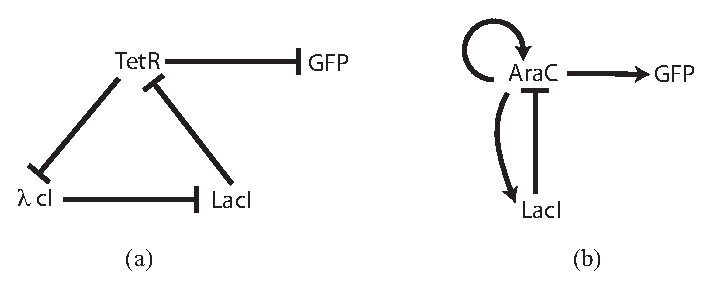
\epsfig{file=figures/oscillators.eps, scale=0.9}
\caption{\label{fig:oscillator}Two different architectures for a
  genetic oscillator. Nodes represent proteins (see
  Chapter~\ref{ch:in-vivo}). Normal arrows mean ``activates the
  production of''. Blunt arrows mean ``represses the production
  of''. (a) A ring oscillator \cite{elowitz-repressilator} called the
  {\em repressilator} consisting of three {\em repressors} connected
  in a ring. (b) A relaxation oscillator consisting of repressors and
  activators \cite{hasty-oscillator}.}
\end{figure}

In synthetic biology, we do not yet know how to build systems that
solve these problems, but we have begun to explore different
architectures for solving specific problems. For example,
Figure~\ref{fig:oscillator} shows two different architecures for
producing oscillations (these are covered in more detail later in this
book). The first is a familar ring oscillator, and the scond is a
relaxation oscillator. Why one would be better than the other in a
given situation will hopefully become clear as we delve into the
details of how they work. 

% The right models and analysis tools
\paragraph{Modeling:} Systems biologists are tempted to write down
equations describing every single reaction in the systems they
study. For example, a recent paper describes a system involving 828
biochemical reactions with 499 ordinary differential equations (ODEs)
with 229 (unknown) parameters \cite{large-model}. This model is fitted
to typically scant data obtained in the lab to obtain estimates of
what the parameters are. The authors also note that the behavior of
the system is insensitive to changes in a number of parameters (taken
one at a time) and infer that as a result they ``know'' some paramters
better than others.

Several fundamental problems with using enormous models are
immediately clear. First, we don't really know good models of even
single reactions inside cells -- their structure is always an
approximate (e.g. is it bimolecular, cooperative, etc.?) and the
reaction rate constants are pretty much impossible to measure. In
fact, the structure of these reactions typically come from what
studies in which a gene is turned off aritifically and the behavior of
other genes is observed to determine causality. When there is
causailty, a reaction is included in the model, whether the
interaction is direct or indirect, fast or slow, etc. Thus, a
collction of even three such ``reactions'', let alone hundreds, is
suspicious. Second, once a system of ODEs is large enough, it is
usually possible to fit almost any finite data set. Therefore, fitting
does not validate or invalidate the model. One may as well fit a
neural network to the data! Finally, modeling and then fitting is
merely {\em descriptive}, not {\em predictive}. A model is really only
useful if it can help you do something (like $F=ma$ helps design
spacecraft trajectories) or makes a scientific prediction that
suggests further experiments.

Many systems biologists are now taking a more pragmatic view of
modeling. One idea, roughly, is to pose the simplist model that both
explains that data at hand and that is useful for predicting data in
new situations\cite{avano}. This is an engineering approach called
{\em system identification} and has been used successfully for decades
outside of biology. Within biology, the approach is viewed with
suspicion: what good is a simple model if it does not account for
every moving part in the system? Another idea is to ask {\em
  qualitative} questions about
networks\cite{zero-deficiency,monotonic-networks}. For example, one
can show that networks without feedback loops are incapable of
oscillating or that there exist a broad set of parameters that do make
another architecture oscillate. This information could be used by the
synthetic biologist to design an oscillator for which there is some
hope of tuning it into place. Yet another approach is to actually
automate the scientific method by designing experiments that are
guaranteed to eliminate as many candidate models as possible
\cite{georgiev-klavins-descrimination}. Such an approach could be
coupled with the design process much as a debugger is coupled with a
compiler.

% Building robust behaviors
\paragraph{Robustness:} Living systems are incredibly robust to
variable nutirent supplies, temperature changes, toxins, mutations,
new competitors, and on and on. Human technologies can be robust too,
or not. Your typical compact car can take all sorts of abuse, but a
the free laser pointer I just got as a freebie at a conference will
probably last about a week before if falls apart. What exactly makes a
system robust is an incredibly subtle question and is asked in all
fields of biology and engineering (in fact, it is one of the primary
questions that brings the two fields together). Control systems
engineering is one of the only fields, however, to actually have
devised a formal, mathematical notion of robustness. Roughly, a system
is {\em robust} to a given {\em perturbation} if its behavior degrades
gracefully as the intensity of the perturbation increases
\cite{robust-control}. Robust behavior in the face of large discrete
changes, however, is still a subject in need of attention.

For synthetic biologists, the most immediate challenge may not be
designing robust molecular systems. Instead, the real challenge is to
understand why and how biological systems are robust. Much of systems
biology concerns this question
\cite{heat-shock,calcium,more-robustness-papers} and successful
explanations there promise to greatly inform the designs of synthetic
biologists.

% Using stochasticity
\paragraph{Stochasticity:} Imagine a computer each of whose bits in
RAM randomly flip from 0 to 1 and from 1 to 0 several times a day
(meaning that the number of flips per second is huge). Such a computer
would have to be programmed very differently than computers
today. Unfortunately, randomness is all over the place in cells. It
arises from several sources. First, because cells are small and
molecules are even smaller, thermal fluctuations are actually quite
large compared with signal intensities. A chemical reaction, for
example, is just a description of the random event that the reactants
happen to combine in just the right geometry to react, the randomness
arising from the giggling and jostling of the reactants and all the
other molecules in the cell. This kind of ``noise'' is called {\em
  extrinsic noise}. Second, the number of molecules of any given type
(called the {\em copy number} of the molecule) inside a cell may be
quite small, say from zero to 50 at any given time. The event that one
of those molecules reacts with another is also a random process. This
kind of randomness is called {\em intrinsic noise}. 

Stochasticity can be readily seen in single cell observations
\cite{elowitz-single-cell}. Isogenic cells with essentially the same
initial conditions can diverge in their behaviors within a relatively
short period of time, due only to the random interactions of the
molecules inside of them. Stochasticity is both compensated for and
exploited by single cells. For example, the process of {\em mitosis}
(cell-replication) has to have very little randomness in it to produce
an essentially identical copy of a dividing cell, and much of the
circuitry responsible for this behavior is presumed to minimize errors
\cite{error-correction-in-mitosis}. On the other hand, randomness may
be used by populations of cells to diversify strategies. For example,
soil bacteria deside to either become {\em competent} (take up DNA
from the environment) or not using essentially a genetically encoded
coin-flipping mechanism \cite{elowitz-b-sub}. The result is that a
precise percentage of a population of such bacteria will be competent,
while others continue to grow. In a fluxuating environment, such a
strategy might be the best bet to ensure survival. (THIS SHOULD BE A
DIFFERENT EXAMPLE). 

Synthetic biologists need to learn to compensate for and use
stochasticity as well. For example, a fundamental question is how does
noise propogate through biochemical reaction networks. If an
intermediate signal is noisy, how is that noise suppressed in the
ouput \cite{avano-noise-cascade}? Also, engineers have found great
uses for random number generators in computer codes (e.g. in
security). How can we make and employ random number generators in
cells?

% Debugging
\paragraph{Debugging:} Electrical engineers use oscilloscpes and
network analyzers to characterize and debug circuits. Computer
scientists use debuggers and runtime analyzers to find bugs. What do
synthetic biologists use? It turns out to be very difficult to
determine what is actually happening is a cell. The information that
is ideally required is a core-dump: we want to know the copy number of
every kind of molecule in the cell as well as its state
(e.g. phosphorylated or not, how it is folded, what it is attached to,
etc). Unfortunately, we can't get this information. But there are
several things we can do. We put GFP and similar reporters (there are
about six colors available) that we can see. We can tag proteins with
molecules that fluoresce in some situations but not in others
\cite{msb-fre-study}. We can take a population of cells and sort it by
size, color, and fluorescence intesnsity \cite{facs}. We can kill the
cell or, more commonly, a population of cells and measure the amount
of RNA or protein to determine which genes were on just before the
cell was killed. We can watch cells grow under the microscope and even
see where certain proteins are being expressed. Every year more
techniques for seeing what is happening inside cells are invented. But
it is likely that we will be in the dark about most of what is going
on inside cells for a good long time. 

Synthetic biologist can respond to this rather fundamental limitation
in a different ways. One idea is to focus on engineering debugger
circuits that could be included in easy to use strains of
bacteria. The idea would be that the cells have built into them
standard debugging tools that can be turned on or off by external
signalling. This is pretty far out, but gives a flavor of what is
really required to do solid engineering with cells. A more down to
earth idea is to carefully ask the question: Given that there are a
limited number of reporter molecules (such as GFP) that can be used at
any given time, where should they be put with respect to a new
proposed design to yield the maximumn amount of information? And more
generally, what information about the behavior of the cell can be
infered from a dynamic trace of those reporter molecules? Recent work,
for example, demonstrates what information can be gleaned from just
the noise characteristics of gene expression
\cite{murray-noise,thorsely-egbert-klavins-in-progress}.

% Preventing systems from being evolved out (Sean's data about # of generations)
\paragraph{Evolution Again:} Recall the discussion above concerning
evolution: It is a fundamental problem in synthetic biology that the
systems we build will be deployed in evolving populations. We desire
two things. One, the systems we build do not get evolved away; and
two, the systems we build do not evolve into something we cannot
control. For the time being, the main problem in synthetic biology is
the former \cite{evolve-away}. Primarily, dropping circuits is a
fantastic strategy for a population since the circuits we so far know
how to design put such an enormous metabolic load on the cell. As we
get better at synthetic biology, expect more graceful circuits that do
not interfere with normal processes. Even then, however, evolving-out
will be a problem. A further improvement is to couple the behavior of
the desired circuit with the very survival of the cell. For example,
suppose that the cell is grown in antibiotics (a ver common way to
test for successful incorporation of a synthetic gene is to also add a
gene encoding for an antibiotic). Next suppose that part of the normal
functioning of parts of the synthetic circuit is to build parts of an
antibiotic protein and assemble it. If any part of the circuit drops
out, the antibiotic is not made and the cell cannot survive. This idea
is similar to the idea of protecting software from being copied or
changed by having it occasionally compute a checksum of its own bits
and aborting if the checksum does not add up.

\section{The Ethics and Risks of Synthetic Biology}

% example: risks of plastic eating bacteria
Synthetic biology has the potential to change everything, for the
better or otherwise. New life forms or new variants on existing life
forms could be dangerous, either accidentally or intentionally. Many
people question whether synthetic biology should be studied at all,
given its {\em dual use} nature. The question is, should we be allowed
to engineer living systems? One answer is, I think, is that {\em we
  already do engineer living systems} -- just not very carefully. 

In fact, we use living systems in a number of ways to positively
impact our health and economy. Bacteria help process nutrients in our
guts and digest waste in landfills. Spiders control insect
populations. Bees pollinate our crops. Algae help supply the world
with oxygen. Exotic trees in the Amazon might produce molecules that
help us treat diseases. It almost seems as if these organisms are in
our service. On the other hand, you can get a tapeworm, bacterial
meningitis, herpes, HIV, the flu, and a whole host of other nasty
problems if you interact with the natural world in an unlucky
way. Furthermore, locusts could eat your crops, termites can eat your
home, or a goose could fly into the jet engine of your airplane to
Boise.

In any case, some of the things we have done technologically and
socially over the last several thousand years have resulted in vast
changes to the natural world that, to date, are far more significant
than changes due to direct genetic tweaking. And the rate at which we
are altering the environment by non-genetic means is increasing. When
the environment is changed and a new niche emerges, some part of the
natural world adapts or possibly collapses – sometimes very
quickly. Examples: The use of pesticides has resulted in new strains
of more virulent pests. The use of antibiotics has resulted in more
virulent strains of infectious bacteria. Our traveling the world in
airplanes has allowed for completely new ways for infectious diseases
to spread. Our use of artificial sweeteners may have made many people
obese. It is very likely that many emerging infectious diseases and
conditions will result directly from new niches that were accidentally
created by for some totally innocuous sounding purpose.

The point is that our current understanding of everything from ecology
to molecular biology is not sufficient for us to begin to evaluate the
introduction of a new policy or technology (even if it does not seem
to be directly related to genetic engineering) in terms of its impact
on the well-being of our species. That is a frightening world to live
in because we are not in control.

Furthermore, nature is designed to manipulate genetic information very
well already. When a population of bacteria finds itself in a new
niche (such as in a moist air-conditioning duct in an office building
or the bilge water of a cargo ship) having strange new nutrients or
surprising new stresses, the population evolves -- often very
quickly. The population of bacteria does this in what seems like a
directed way, but it is really ``just'' evolution. Now, evolution is
simple to describe, but it can move in surprising directions in
seemingly deliberate ways as we discussed above. While still “obeying”
the laws of evolution, bacteria have evolved techniques to evolve
quickly and without merely randomizing their genomes. For example, a
recent paper in Science showed that when a population of {\em
  Streptococcus pneumoniae} is subjected to antibiotics, the bacteria
in the population begin to share DNA among each other
\cite{strep-evolve}!  This allows each bacterium in the population to
try out new genes to fight antibiotics like you might try out a new
piece of shareware from the Internet to combat adware.

We are surrounded by many other examples of rapidly evolving organisms
that seem to have a greater facility with genetic engineering than we
do (they are better at directed exploration to be more exact). HIV and
avian flu evolve very quickly within each host they infect, thereby
adapting to the host and possibly to a treatment regimen. What’s more,
microorganisms evolve much more quickly than we do as a species
because their life spans are shorter. In contrast to humans, who seem
to be at the mercy of their biological environment, the natural world
is actually very adept at surviving and even flourishing in the face
of dramatic changes and attacks.

But our technology evolves for us. Computers evolved from massive,
single purpose beasts the size of buildings to sleek personal digital
assistants that inhabit our pockets (the PDA is just one family of
computer among many flourishing today). Automobiles, agriculture,
buildings, financial markets, power plants, warfare, chewing gum, and
arthritis drugs have all undergone similar evolutions from crude
beginnings. All of these technologies augment (or at lease change) our
ability to survive in the natural world. Not much about us genetically
speaking enables us to live in almost every part of the globe (except
our brains). It is our technology and accumulated knowledge that
enables us to survive mat present levels. Our technology is now
allowing us to re-program living systems directly -- which is a
fundamental shift in the place of humanity in the universe. 

If technology is truly subject to
mutation and selection, then its development is essentially a random
process. New technologies are developed, by engineers, based on old
ones that work well. Customers use products that serve their current
needs. Old technologies become obsolete and eventually extinct. Even
better, our technology is co-evolving with us and with other life
forms on our planet. However, just as biology is more likely to move
in some directions than others, we ourselves can, to some extent,
control the direction that our technologies evolve (with policy and
planning). By better understanding the natural world and our place in
it, we can develop technologies that make us safer, healthier, and
happier. Synthetic biology is hopefully one of those technologies.

Of course, any sufficiently new and powerful technology has risks that
need to be understood and managed. One of the startling aspects of
synthetic biology (which is also what makes it fun to study) is that
new potential applications (safe or otherwise) seem to pop up every
day. Therefore, we simply do not know what we (or someone else) will
be able to build tomorrow. Furthermore, the technology required to
build something new in this field is suprisingly simple, making it
available to anyone. How the uses of synthetic biology should be
regulated is a difficult and open question. Two most-likely unworkable
ideas present themselves. First, synthetic organisms could be
regulated like toxic chemicals. Second, synthetic organisms could be
regulated using the existing bio-safefty regulations for infectious
agents (from {\em Salmonella} to the 1918 flu). Only laboratories
capable of confining such organisms would be allowed to work on
them. Both of these options are problematic because they view the
organisms as the risk. In fact, it is the information -- merely a
sequence of $A$, $T$, $C$ and $G$s -- that really defines a life
form. Technologically, we are close to the day when almost anyone will
be able to boot up a new organism starting only with the genetic code
defining it.

Thus, what really needs to be considered, is how to keep track of the
information, the code, and thre recipes of synthetic biology. A good
analogy is with computer viruses. If you look up computer viruses on
the Internet, you will find all sorts of descriptions on how to make
them. Furthermore, you can find manuals on how to program in a variety
of languages, and specifications of network protocols and operating
system APIs to help you write very cool Internet applications, and
also very nasty computer viruses, worms, trojan horses, and the
like. The equivalent information for living systems is now being
generated, compiled, and disseminated. But it is one thing to bring
the Internet down, and another to bring the biosphere down.

Thus, among the goals of synthetic biology should probably be to (a)
to understand in what ways synthetic biology is the same and different
from existing bio-technologies so that it can be regulated; and (b) to
understand how to recognize or test for the potential impact of a new
technology on exiting life. The latter requires really a new,
quantitative (and I would argue, engineering-based) understanding of
living systems.

\section{Overview}

This text is an attempt to provide a foundation for the design,
modeling, and analysis of synthetic biological systems. It focuses
primarliy on aspects of dynamical systems and control. The goals are
essentially: (1) introduce the theoretical issues of synthetic biology
to students studying control engineering; (2) introduce control and
dynamical systems to students studying synthetic biology; (3) to
prepare students to understand the research in the area so that they
can begin to contribute to the field. The text does not cover many
other very important issues in synthetic biology, such as experimental
techniques, or logic and computer science. We are preparing a
laboratory manual the {\em does} introduce basic genetic engineering
with bacteria, that is available online.

We assume a minimal background in dynamical systems (basic
differential equations, linear algebra, and probability) and
essentially no background in biology -- although an undergraduate
course in biochemistry would be very helpful. 

The topics included in the text are geared toward understanding the
behavior of systems that researchers have actually built or systems
found in nature that have been well characterized. The goal is to
focus on systems that have some hope of being implemented and the
theoretical issues associated with getting them to work -- as opposed
to more speculative ideas and architetures that are (presently) only
of abstract interest.

Therefore, the topics include the following. First, we give a very
high level overview of the operation of procaryotic cells to ground
the discussion of specific systems later. We give an overview of
synthetic biology {\em in vitro}, as an alternative experimental
reality. There is a breif review of differential equations, mostly to
remind the reader and set notation. Then we discuss the main models
used in systems and synthetic biology, namely mass action kinetics,
enzyme kinetics and stochastic kinetics. The approach to enzyme
kinetics is somewhat different than in other texts in that we first
introduce the {\em singular value perturbation} method from nonlinear
systems, and then show how to apply the method to mass action kinetics
models to obtain enzyme kinetics models. We also discuss the potential
for the misuse of enzyme kinetics models.

As discussed above, models in synthetic biology are to be viewed with
suspcion, primarily because there are no well-established first
principles from which to derive models. Typically the theory of
chemical kinetics is applied to the reactions inside a cell, but the
assumptions required by chemical kinetics are not really met
(well-mixedness, point mass molecules, 3D difussion, etc.). Therefore,
we describe how to evaluate how good a model is and how to obtain
models from data. In particular, we discuss the composition of systems
and what can go wrong; robustness and sensitivity; and parameter
estimation and system identification.

\section{Problems}

\begin{exercise}
  Recall the five capabilities we associate with living systems:
  sensing, actuation, control, information storage, and
  evolution. Which of these capabilities does a car have? How is the
  capability instantiated? What other technologies have these
  capabilities?
\end{exercise}

\begin{exercise}
  Visit the {\em Kyoto Encyclopedia of Genes and Genomes} at
\begin{quote}
  \ \\
  \href{http://www.genome.ad.jp/kegg/}{\tt http://www.genome.ad.jp/kegg/}
  \ \\
\end{quote}
  and search for ``butanol''. Find where
  it says ``Compound'' and click on the first compound. Then click on
  the pathway for Butanoate metabolism. If you have a microorganism
  that synthesizes Butanoyl-CoA, enzyme could you use to
  get Butanoate? What organisms could you get the gene for this
  enzynes from (an exhaustive list is not required)?
\end{exercise}

\begin{exercise}
  Describe a technology with which you are familar. In what ways is it
  robust? In what ways is it fragile? How have designs of the
  technology evolved to become more robust? 
\end{exercise}

\begin{exercise}
  Look up the {\em International Genetically Engineered Machine}
  (iGEM) competition using your favorite search engine. iGEM is a
  synthetic biology competition for undergraduate teams. Look over the
  team wikis from years past and find (a) a medical application; (b) a
  biofuel application; (c) a components-based (e.g. genetic logic
  gates, amplifiers, etc) project. Describe each project briefly and
  speculate what engineering principles might be brought to bear on
  the problem.
\end{exercise}

\begin{exercise}
  Look up the {\em Obligation of the Engineer} using your favorite
  search engine. It describes what responsibilities engineers have
  when practicing their art. How could this oath be changed into an
  {\em Obligation of the Synthetic Biologist}?
\end{exercise}